%\chapter{Case Study 2: BALROG for LLM Reasoning and Reflection}\label{chap:balrog}
\chapter[Case Study 2: Reasoning and Reflection]{Case Study 2: BALROG for LLM Reasoning and Reflection}\label{chap:balrog}

\begin{learningbox}
In this case study you will gain hands-on experience building self-reflective agent for  reasoning domains. 
Specifically, you will be able to:
\begin{itemize}[leftmargin=*, nosep]
    \item Run a multi-step {\em reasoning agent} on a benchmark of puzzles and games.
    \item Adapt a reasoning agent with your own ideas.
    \item Implement your own {\em self-reflective} agent.
    \item Critically reflect on the {\em performance and stability} of a learning agent in the domain of puzzles and games. 
\end{itemize}
\end{learningbox}

\section{BALROG Overview}
%We will discuss a practical 
In this case we will work with an agentic LLM that  performs self-reflection. We use a popular benchmark suite for reasoning tasks, called BALROG.\footnote{A Balrog is a mythical demon from Middle-earth, featured in the fantasy works of J.R.R. Tolkien. A Balrog is a match even for Gandalf the Grey, the most powerful wizard of  all.} BALROG is an acronym for {\em B}enchmarking {\em A}gentic {\em L}LM and VLM {\em R}easoning {\em O}n {\em G}ames. The BALROG benchmark consists of a mix of easy and hard games, some of which are difficult for LLMs to play well, as the BALROG paper shows in their own benchmarking study \citep{paglieri2024balrog}. 

Initially, the BALROG games are benchmarked with vanilla LLMs. The code, however, is quite open and amenable to writing your own agent approaches, to see if you can do better.
%The BALROG suite is designed in a way to invite others to use it. 
The software is written for you to write your own agent code for in-context (reinforcement) learning. 



%In this chapter we will use the BALROG  benchmarks to experiment with the reasoning and self reflection  approaches that we discussed in the previous  chapters.

\begin{comment}
    

\section{Learning Goals}
The  goal of this chapter is to better understand the  capabilities reasoning models and self reflection mechanisms, and their weaknesses. This experience will help you understand the challenges faced when designing reasoning and self-reflection agents for your applications.


After completing this case, you should be able to:
\begin{enumerate}
    \item Implement an agentic LLM system with explicit planner and executor roles
    \item Run the agent on challenging plannign-type problems
    \item Evaluate, debug and analyze experimental results
    \item Critically reflect on the capabilities of reasoning agents on challenging puzzle and game benchmarks
\end{enumerate}
\end{comment}



The main BALROG website is  \url{https://balrogai.com}.
%The system  can be found onGithub \url{https://github.com/balrog-ai/BALROG}. 
%
The code is  easy to adapt and use for your own experiments, and there is a leaderboard. In this chapter we will guide you to write your own agent code, that can then be run on the BALROG games-suite. 

\begin{figure}[t]
    \centering   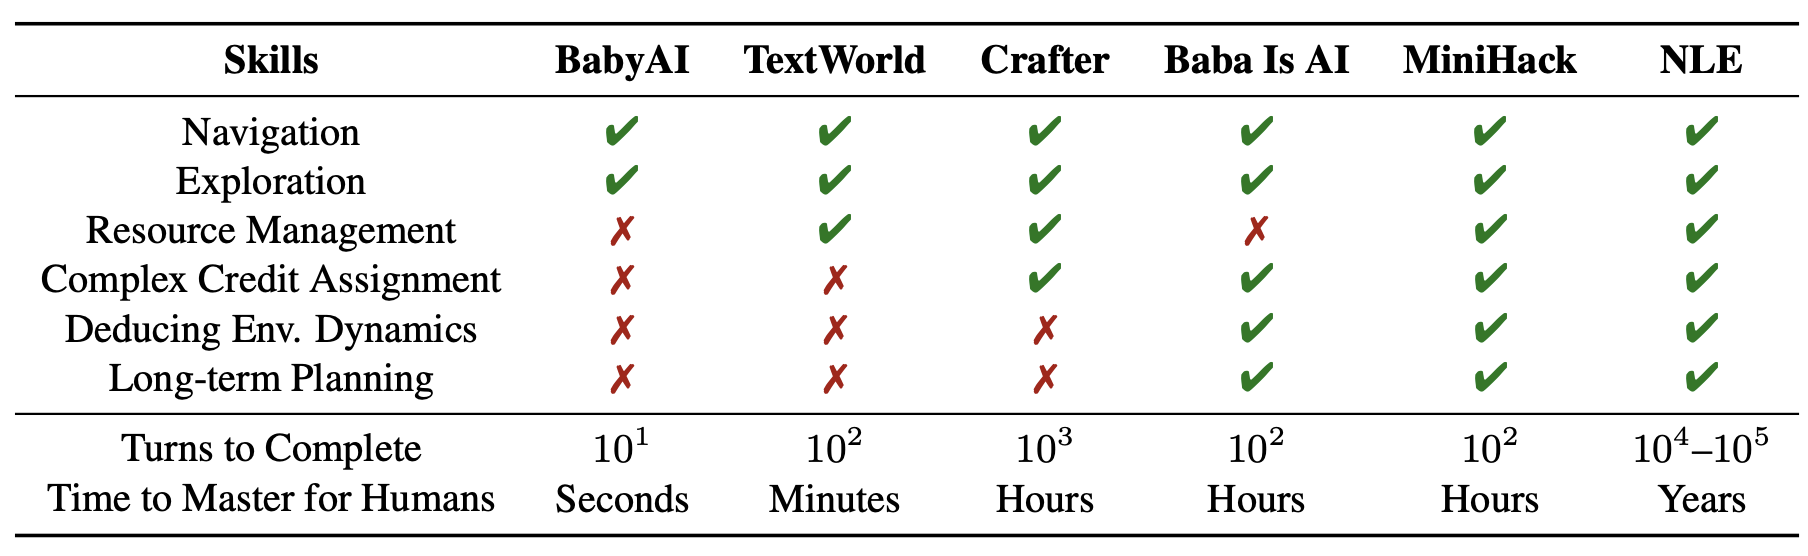
\includegraphics[width=0.98\linewidth]{figures/balrog}
    \caption{List of games in BALROG \citep{paglieri2024balrog}}
    \label{fig:balrog}
\end{figure}

BALROG is designed to challenge in-context agents on reasoning problems.
It uses puzzle-style games to benchmark the reasoning capabilities of LLMs and VLMs. Figure~\ref{fig:balrog} lists the games. The games are from easy to hard: BabyAI, Crafter, TextWorld, BabaIsAI, MiniHack, and NetHack. The games offer a mix of challenges, some are text-based, some have a visual component, all include reasoning challenges for the model. Some of the games are considered hard. For example, it is not expected that your model or your agent---or your self---will reach a high score on NetHack. (If you do achieve that, without having accessed the cheat-sheets, you may want to consider writing a paper for a prestigious AI conference.)

\begin{comment}
BALROG is designed originally for in-context learning, where the agent is simply a prompt improver (such as Tree of Thoughts or ReAct). 
Only inference is necessary. However, some of the BALROG games are quite challenging. Nothing prevents us from going to the next level and to try metalearning, or finetuning, such as GRPO, RLVR, or ReFT. These advanced methods are for later, however, we will start with regular in-context learning.




\paragraph{Multi-step Reasoning}
In agentic LLM, we want our agents to be able to communicate in natural  language, but they should also be able to make intelligent decisions, to reason and to look ahead about the consequences of their actions. Reasoning benchmarks test these abilities. Many games make excellent benchmarks to test if an agent can do multi-step reasoning well. 

The games in BALROG are quite diverse: some are easy, some are hard. They allow us to test if chain of thought prompts are powerful enough to solve easy planning problems, and hard planning problems.

\paragraph{Self Reflection}
As we have seen in the previous chapters, chain of thought is sometimes not strong enough, and we want our agent to learn from its mistakes, to be able to self-reflect, to see if its reasoning should be adapted.

This brings us to metalearning, the problem of learning to solve a set of {\em tasks}, instead of just a set of examples (a single task).

%First of all we can see self improvement of the policy of actions, a single level of learning. You can also go a level higher, to metalearning, to try to improve the learning algorithm, as we saw in the last chapter. 

Before we jump into metalearning right away, we should first get a single level baselearner to work well, bug free, achieving stable learning, giving results that fit our intuition. 
Only if we have a stable baselearner whose behavior you understand, does it make sense to try to build a second level of learning on top of the baselearner. %The proverb about running and walking applies.
\end{comment}

\subsection{Puzzles and Games}
BALROG  consists of the six puzzles and games shown in Figure~\ref{fig:balrog}. The games run from easy grid world puzzles to hard text-based dungeon and dragons strategy games, with long credit assignment episodes and flat reward landscapes.

The authors of BALROG provide a code base that allows experimentation with agents, to design your own agent, to see how well they do on the benchmarks. To perform well on the benchmarks in BALROG, the agents must be good at reasoning and planning, and, most likely, be good at adapting and reflecting on their own behavior. 


%Well suited for reasoning, testing planning capabilities of LLMs.

%* describe balrog: benchmark suite, puzzles and games, planning challenge


BabyAI is a simple grid-world game, where the agent has to solve a navigation task. A simple reinforcement learning type algorithm would be able to easily solve this game. Tasks are given in natural language, such as: {\em go to the blue ball, then pick up the grey key}. Of course, the challenge for the agentic LLM is to perform the planning part of the task. It is expected that the LLM will be able to do well on this simple game (see the BALROG paper). 

NetHack, on the other hand, is a highly challenging game, also for human players. NetHack is a text-based dungeons and dragons-like game. It includes both
long-term strategic planning, in the sense that winning a game can involve hundreds of thousands of steps, and  short-term tactical fights to fend of the usual hordes of monsters. Credit assignment is  a challenge in NetHack, in order to  understand which of the actions that the agent took in the past contributed to ultimate success or failure, since actions in one area of the game may have unexpected consequences far away, making it difficult to play for reinforcement learning agents. NetHack is known for  human players to take years to
master the game without resorting to cheat guides.

\begin{comment}
    
\subsection{Knowing-Doing Gap}

As we discussed in Section~\ref{sec:knowing},  LLMs are often able to {\em answer} questions about the game mechanics and optimal strategies (the cheat guides were presumably part of the pretraining corpus), but they often
fail to be able to  apply this knowledge in practice.  This phenomenon has been called the {\em knowing-doing gap}. An LLM may be able to recite an algorithm to solve a problem, but it is not able to correctly execute this same algorithm.  The knowing-doing gap occurs in the harder puzzles, where the agent is not able to execute planning and reasoning to the required level of precision. It starts making errors. LLMs are good at associative lookups, not at precisely keeping track of changes to the values of variables. See also Section~\ref{sec:knowing}.


For you, in your experiments,  the challenge is to see if you can get your system to work well enough that you can run (moderately) difficult problems, so that the knowing-doing gap  occurs, and, then, of course, if you can find a way to make your agents  overcome the gap.

\end{comment}

\begin{figure}
    \centering
    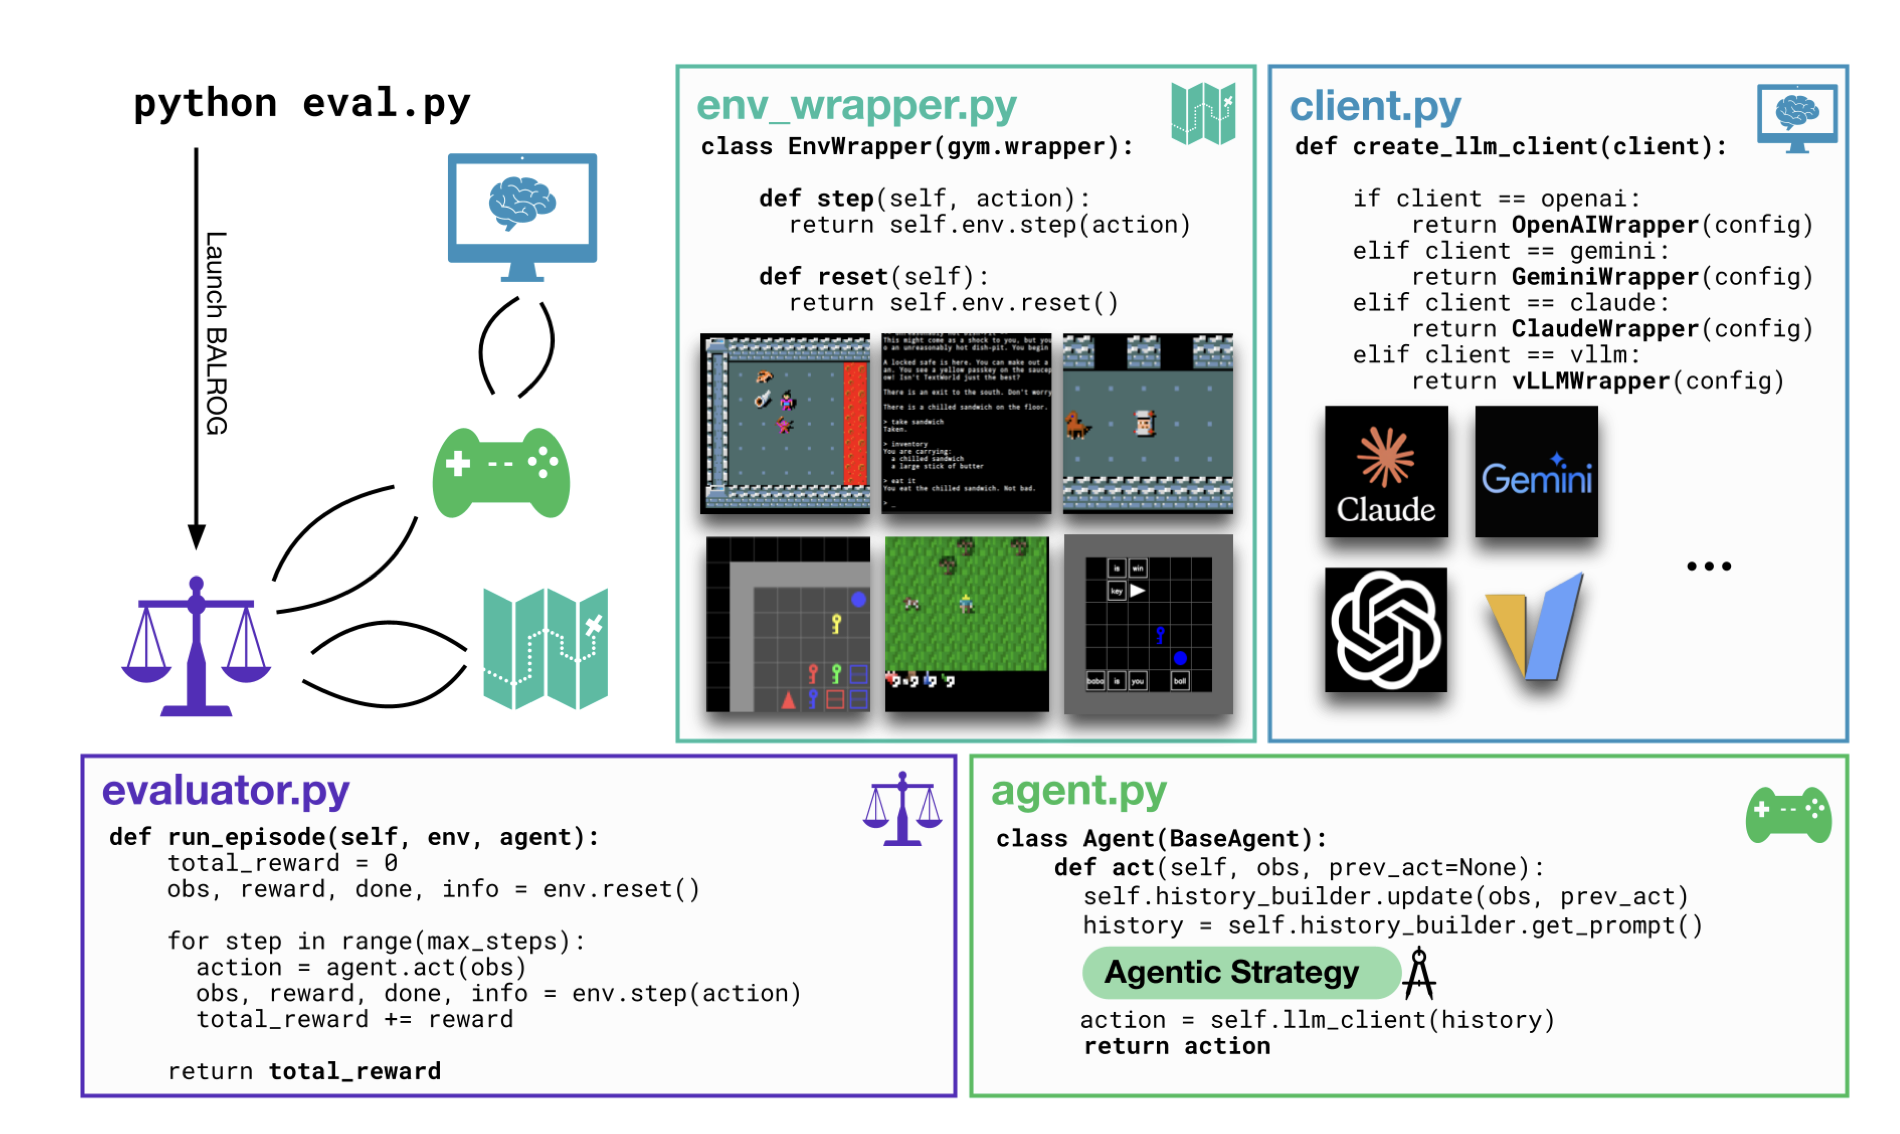
\includegraphics[width=\linewidth]{figures/balrogarch}
    \caption{Architecture of BALROG \citep{paglieri2024balrog}}
    \label{fig:balrogarch}
\end{figure}

\subsection{BALROG Architecture}
We wil now have a look at the architecture of the BALROG framework. Figure~\ref{fig:balrogarch} shows the architecture, taken from the paper \citep{paglieri2024balrog}. 


%\subsection{Read Paper}
% - read paper to understand balrog goal \citep{paglieri2024balrog}.

Please familiarize yourself with the BALROG system. Read the paper \citet{paglieri2024balrog}, which you can find on \url{https://arxiv.org/abs/2411.13543}, or go to the BALROG website at \url{https://balrogai.com}. %(Many good papers in machine learning provide the code with their papers on Github, to ease reproducibility of their work.)


If you have not done so yet, install BALROG on your system with the \verb|git clone| command.  
Go to \url{https://balrogai.com}, or directly to the Github repository at \url{https://github.com/balrog-ai/BALROG}. Install the repository on your local computer.

Decide which LLM you want to use. Please note that typical BALROG agents make many LLM calls, at each step of the way. If you want to run the LLM locally, install it, or use it from Huggingface. If you want to use a (commercial) cloud-based LLM, acquire an API-key and install the API-key in your environment. You may want to consider applying for a free student-tier, if that is offered. The use of frontier LLMs can be expensive, but usually older and smaller LLMs, some of which are still relatively capable, are much cheaper.

The BALROG readme on the Github repository contains information on how to install the system, and how to install an API key for your favorite LLM, see Listing~\ref{lst:key}. (In one of the exercises we will use multiple LLMs, to compare their performance. For now, we are just trying to get the system to run, and anyone will do.)
\begin{listing}
    \begin{minted}[
frame=lines,
framesep=2mm,
baselinestretch=1.0,
fontsize=\footnotesize,
linenos
]{bash}
        export OPENAI_API_KEY=<KEY>
        export ANTHROPIC_API_KEY=<KEY>
        export GEMINI_API_KEY=<KEY>
    \end{minted}
    \caption{Installing the API key}\label{lst:key}
\end{listing}

\subsection{Agent}
Please read the Agent tutorial in BALROG at \url{https://github.com/balrog-ai/BALROG/blob/main/docs/agents.md}. In BALROG, agents are small pieces of Python code that call  an LLM with a prompt to provide an answer how to determine the next step. The agent code is  responsible for receiving answers from the model (observations) and for  selecting the next action. The LLM is used to execute various prompts.  

BALROG follows interaction style D from Figure~\ref{fig:rlD},  where the prompt is built up from the history of interactions. 

\subsubsection{Prompt Builder}
The agent builds  a prompt based on previous actions, based on observation/action pairs from previous interactions. 
Thus, in reinforcement learning terms, the agent performs the function of the policy, selecting the next action to perform based on the incoming observation. 

Go to the \verb|prompt_builder| directory to change the way that prompts are constructed from the history of actions. 

\subsubsection{Agents}
Agents are responsible for the memory function: managing 
the observation/action histories. 
The agents must keep a record of past observations and actions to support context-aware decision-making, and this must be implemented by us, external to the LLM.

The agent code in BALROG queries  the LLM: agents send observations to the LLM, receive responses, and use those responses to decide on actions to take in the game.

BALROG comes with a number of pre-written agents, which you should study to design your own. The repository has a naive agent and a chain of thought agent. Also provided are more robust versions for handling LLM responses. 

When you build your own agent, you will most likely build on the custom agent. 
The BALROG agent tutorial provides an example for a simple planning agent.


\section{Implementation Steps}
We will now provide some exercises to help you explore building your agents.
\subsection{Reproduce Paper}
%- task 1: implement standard task, reproduce.

We start by trying to reproduce the results in the BALROG paper.
Please have a look at the BALROG code at Github \url{https://github.com/balrog-ai/BALROG}. Read the Evaluation Guide, the Agent Development tutorial, and the instructions how to run Few Shot Learning experiments (in-context learning).
Install the relevant tools on your computer, and the right Python version (and put it in your PATH). Check the version by starting the Python interpreter from the command prompt: \verb|$ python|.

First, run the standard evaluation, to make sure you installed things correctly, see Listing~\ref{lst:eval}. 
\begin{listing}
    \begin{minted}[
frame=lines,
framesep=2mm,
baselinestretch=1.0,
fontsize=\footnotesize,
linenos
]{bash}
 python eval.py \
  agent.type=naive \
  agent.max_image_history=0 \
  agent.max_text_history=16 \
  eval.num_workers=16 \
  client.client_name=openai \
  client.model_id=gpt-4o-mini-2024-07-18       
    \end{minted}
    \caption{Running the standard evaluation}\label{lst:eval}
\end{listing}




\subsection{Different LLMs}
%- task 2: try different models, run local/api, use wandb.ai, setup extensive experiment chain

To get a feeling for how the standard agent performs on the different benchmarks with different LLMs, it is useful to run a few different LLMs. %When you are using the API version, this requires acquiring different API keys, which may cost you money, or finding out which free tiers for students are possible. 
It is  recommended to run closed and open LLMs, and see how they perform. Especially the open version from OpenAI, Claude, DeepSeek, OLMo and Qwen may work  well. 

Running these models is important, and  will lead to more insight into the relative strengths of the various models.

\subsection{Different Puzzles}
%- task 3: try different puzzle problems, understand the problems
Next, to get a better understanding of the benchmark, you should, after running the LLM agent in the different puzzle problems, have a closer look at the prompts and the answers of LLM. See if you can see where the LLM agent fails, where the weakness of the agent lies. By close inspection of the individual actions, and a deeper understanding of the puzzle, you might be able to think of a way to improve your agent.

\subsection{Computational Cost}
BALROG agents call an LLM for each step that the agent makes, often with a long prompt. In these puzzles and games many such steps are made. Running  different LLMs on the full benchmark, for different seeds, will easily require  many tokens. 

In your experiments, first try a small and cheap LLM, such as  Qwen-3B. Start with the easiest benchmarks (BabyAI and Crafter). If you wish to expand, please go ahead, but be mindful of the computational cost. You want insights, but you also want your experiments to finish in a reasonable time for a reasonable cost.

\subsection{Implement Own Reasoning Agent}
%- task 4: implement own agent, baselearner. 
Now it is time to implement your own learning agent.
Go to the agents directory in balrog, and edit the \verb|custom.py| file.
Listing~\ref{lst:agent} reproduces the code for Custom Agent from the BALROG readme. The code can be run with the command in Listing~\ref{lst:agent-run} (specifying the custom agent, and running gently with fewer workers). Of course, you can specify your own LLM of choice in the command.

Start with the provided code, run it, see how it works. Then, you can try to make small improvements. Try making changes to the prompt for the LLM, and to the way in which the Python code handles the learning in the agent, either with the history prompt builder,  in the plan, or in the learning algorithm.

\begin{listing}
\begin{minted}[
frame=lines,
framesep=2mm,
baselinestretch=1.0,
fontsize=\footnotesize,
linenos
]{python}
from balrog.agents.base import BaseAgent
import re


class CustomAgent(BaseAgent):
    def __init__(self, client_factory, prompt_builder):
        super().__init__(client_factory, prompt_builder)
        self.client = client_factory()
        self.plan = None

    def act(self, obs, prev_action=None):
        if prev_action:
            self.prompt_builder.update_action(prev_action)
        self.prompt_builder.update_observation(obs)

        plan_text = f"Current Plan:\n{self.plan}\n" if self.plan else "You have no plan yet.\n"

        planning_instructions = """
Review the current plan above if present. Decide whether to continue with it or make changes.
If you make changes, provide the updated plan. Then, provide the next action to take. 
You must output an action at every step.
Format your answer in the following way:
PLAN: <your updated plan if changed, or "No changes to the plan." if the current plan is good>
ACTION: <your next action>
        """.strip()

        messages = self.prompt_builder.get_prompt()
        if messages and messages[-1].role == "user":
            messages[-1].content += "\n\n" + plan_text + "\n" + planning_instructions

        response = self.client.generate(messages)

        # Extract the plan and action from the LLM's response
        plan, action = self._extract_plan_and_action(response.completion)

        # Update the internal plan if it has changed
        if plan != "No changes to the plan.":
            self.plan = plan

        # Save the plan in the response.reasoning field and the action in response.completion
        response = response._replace(reasoning=plan, completion=action)
        return response

    def _extract_plan_and_action(self, response_text):
        plan_match = re.search(r"PLAN:\s*(.*?)(?=\nACTION:|\Z)", response_text, re.IGNORECASE | re.DOTALL)
        action_match = re.search(r"ACTION:\s*(.*)", response_text, re.IGNORECASE | re.DOTALL)

        plan = plan_match.group(1).strip() if plan_match else "No changes to the plan."
        action = action_match.group(1).strip() if action_match else None

        return plan, action
\end{minted}
    \caption{Agent code in BALROG}\label{lst:agent}
\end{listing}

\begin{listing}
    \begin{minted}[
frame=lines,
framesep=2mm,
baselinestretch=1.0,
fontsize=\footnotesize,
linenos
]{bash}
python eval.py \
  agent.type=custom \
  agent.max_image_history=0 \
  agent.max_history=16 \
  eval.num_workers=64 \
  client.client_name=openai \
  client.model_id=gpt-4o-mini-2024-07-18        
    \end{minted}
    \caption{Running the Agent  evaluation}\label{lst:agent-run}
\end{listing}

\section{Evaluation}
The performance of your agent will be reported by BALROG as a progression percentage. Record the progression numbers for each benchmark, and for the agent types that you try. Do this in a structured way, you may want to write a Python or shell script to automate the running of the experiments and the logging of the results, perhaps also plotting the progression in a graph. Consider using wandb.ai.

What agent types work well, and on what benchmark do they work well? Make a matrix in which you log progression for the agent types and the benchmark types that you try.

Note that LLM experiments are inherently non-deterministic: two runs with the same prompt may give different results. Therefore, perform multiple runs of each experiment. If you get five identical results in a row, you may start to trust these results. If they vary widely, you may want to investigate. Is the reason purely statistical? Does turning down the temperature solve the problem, or is there another problem?

Do not blindly trust the progression numbers that are reported. Since you are using code on a computer, there may be bugs, or other issues. The BALROG system facilitates delving deeper into the runs. It logs csv files that you can look at with a spreadsheet. Have a look at some of the runs, and decide if it makes sense what you see, or if the agents are exhibiting degenerative behavior. If they do, try to find the reason. Did you do something wrong? Is there unexpected interference between the benchmark and the agent behavior?
Is the reward landscape too flat, so that there is no signal for the agent to go after, and all it does is random actions running in circles in a way that makes no sense at all? Is there something that you can do about this?

Please note that the field of large language models, and especially of agentic LLMs, is new, and our insights and our software frameworks have not yet stabilized. Some unexpected results are to be expected, and some challenges or frustration as well.

A structured way of experimentation and result-logging is your friend. Planning and organization can make the running, evaluation, and improvement of practical agentic LLM experiments an enjoyable exercise. 

\section{Self-Reflection}
When you were able to reproduce the benchmark results, and have experimented somewhat with the agents, you may want to try to take on some larger challenges. In this section, we will try to extend the BALROG agent towards self-reflection, where the LLM is used in different roles, such as evaluation and action selection. Self-reflection, as any adaptive system that chases a target that is itself being optimized, can be prone to instability and oscillations. Therefore, before we  try  our self-reflective ideas, it is important that the base learner system of the previous subsection works, and converges in a stable and predictable manner.
Please go back to that section and make sure things work as you want them to work.

There are many recent works that try to improve LLM agents. We will mention two: ReAct \citep{yao2022react} and reflexion \citep{shinn2024reflexion}. ReAct is primarily focused on prompts, where reflexion introduces new agent algorithms, including short-term and long-term memory. 

\begin{figure}
        \centering
    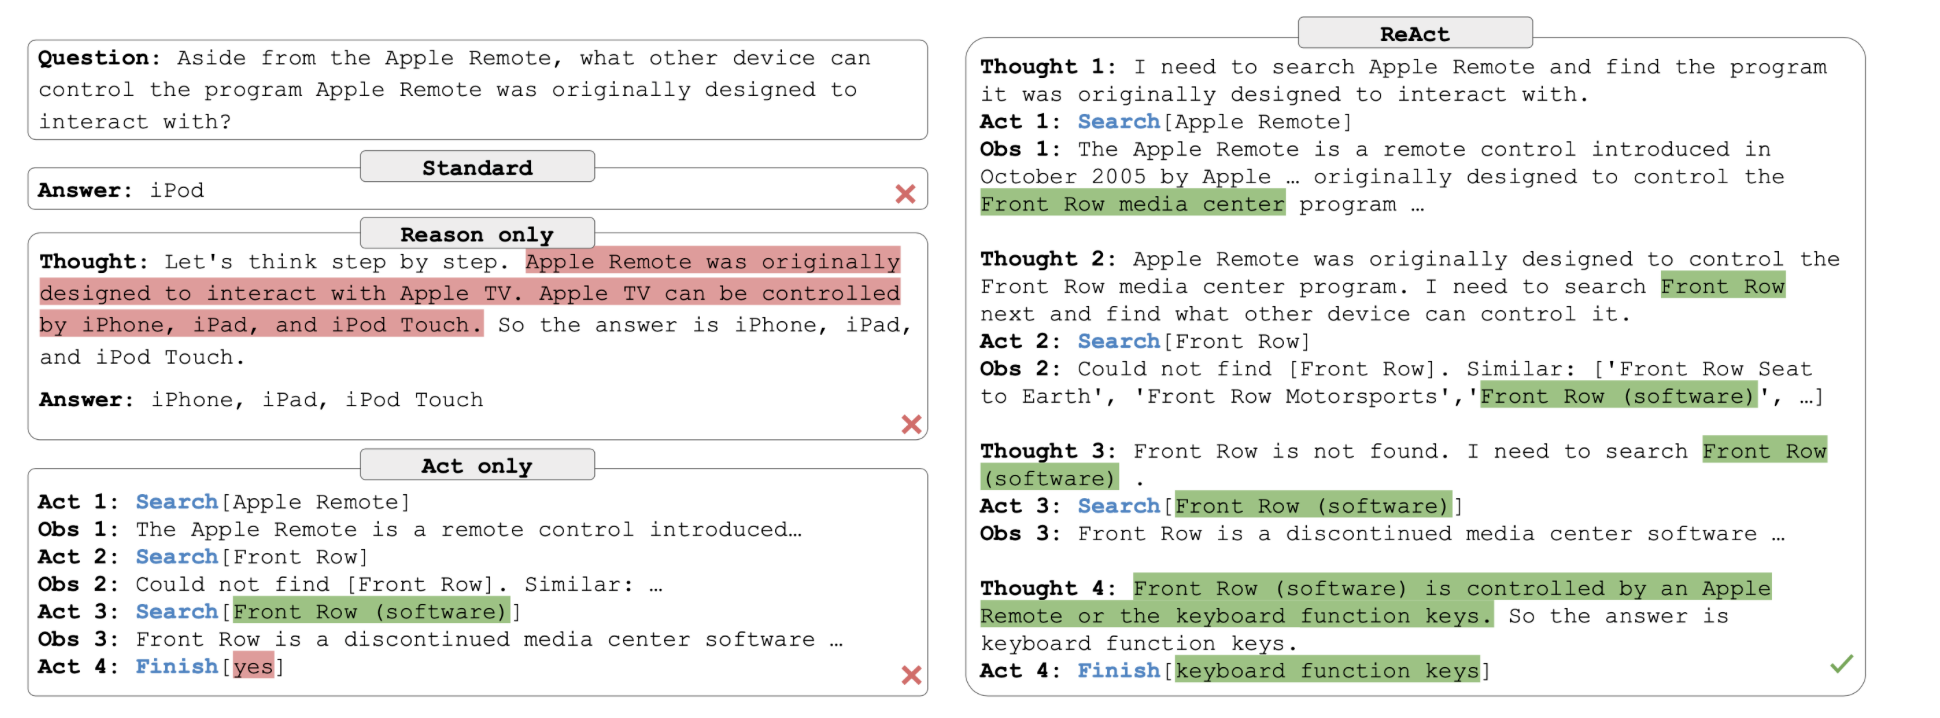
\includegraphics[width=0.95\linewidth]{figures/react}
    \caption{ReAct example Performing Search \citep{yao2022react}}
    \label{fig:react}
\end{figure}

\paragraph{ReAct}
ReAct uses promtps to interact with the world.  ReAct promotes the use of tools, to lookup information, see Figure~\ref{fig:react}. The original website for ReAct is \url{https://react-lm.github.io}, the code repository is here: \url{https://github.com/ysymyth/ReAct}. ReAct prompting has also been implemented in the LangChain\footnote{See \url{https://docs.langchain.com/oss/python/langchain/overview}} and BeeAI\footnote{See \url{https://github.com/i-am-bee/beeai-framework/blob/main/python/examples/agents/react.py}} frameworks. 

Have a look at these framework to get an understanding of the prompt-based agent interaction style that ReAct introduces. Then, implement the prompt-based interaction in BALROG. Does is improve performance? For which games does it help to lookup external information? For which games not?

%- task 5: try self reflection. 

\paragraph{Reflexion}
Where ReAct is prompt-based, allowing interactive lookups, the reflexion approach introduces  Python-coded agents, allowing  more elaborate agent behavior. 
Reflexion uses the same LLM in different contexts, with different prompts.  
It works on the assumption that it is easier to criticize what is wrong with an existing prompt, than to come up with one that works.

Reflexion is a popular self-reflection architecture \citep{shinn2024reflexion}. The main webpage for reflexion is \url{https://github.com/noahshinn/reflexion}. A blog post on reflexion, describing the main ideas, is here: \url{https://nanothoughts.substack.com/p/reflecting-on-reflexion}.

\begin{figure}
    \centering
    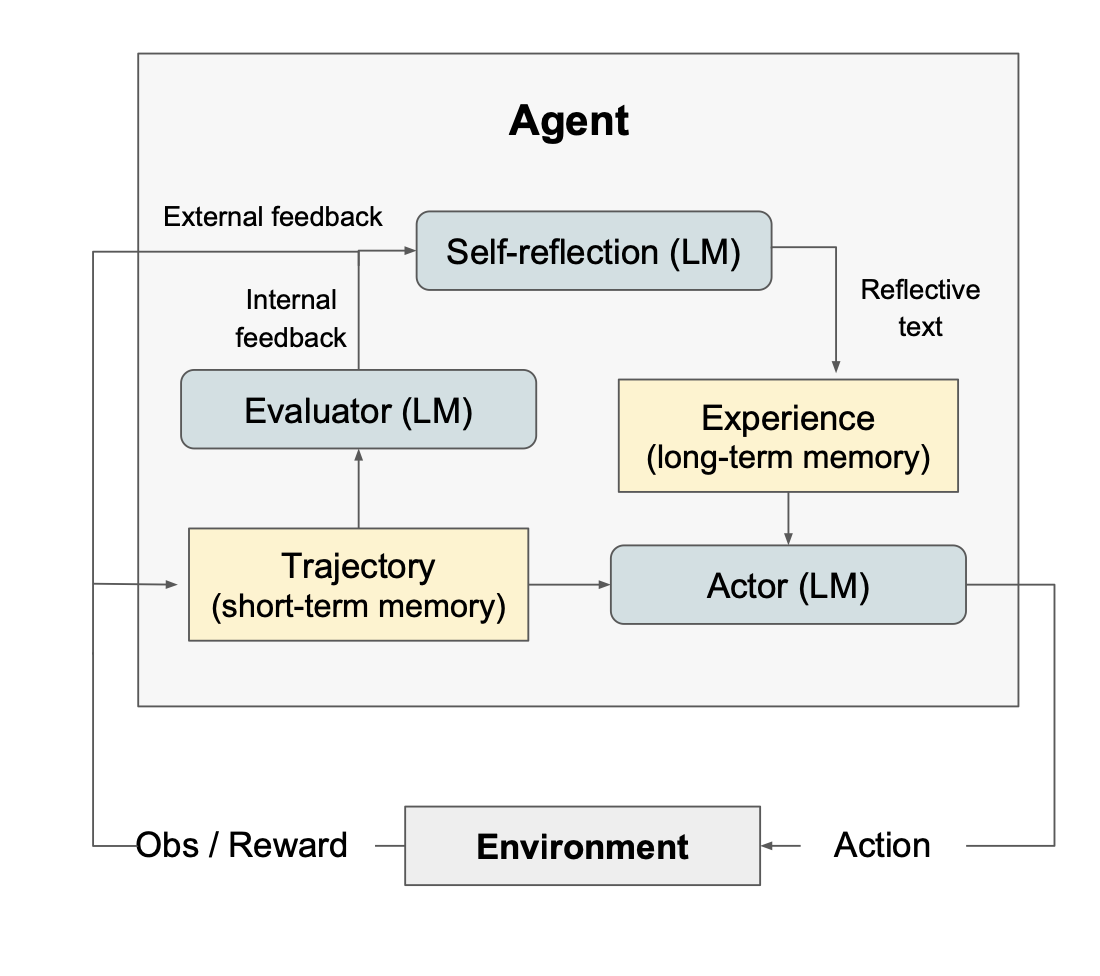
\includegraphics[width=0.5\linewidth]{figures/reflexion3.png}
    \caption{Reflexion Architecture \citep{shinn2024reflexion}}
    \label{fig:reflexion-alg}
\end{figure}


\begin{figure}
    \centering
    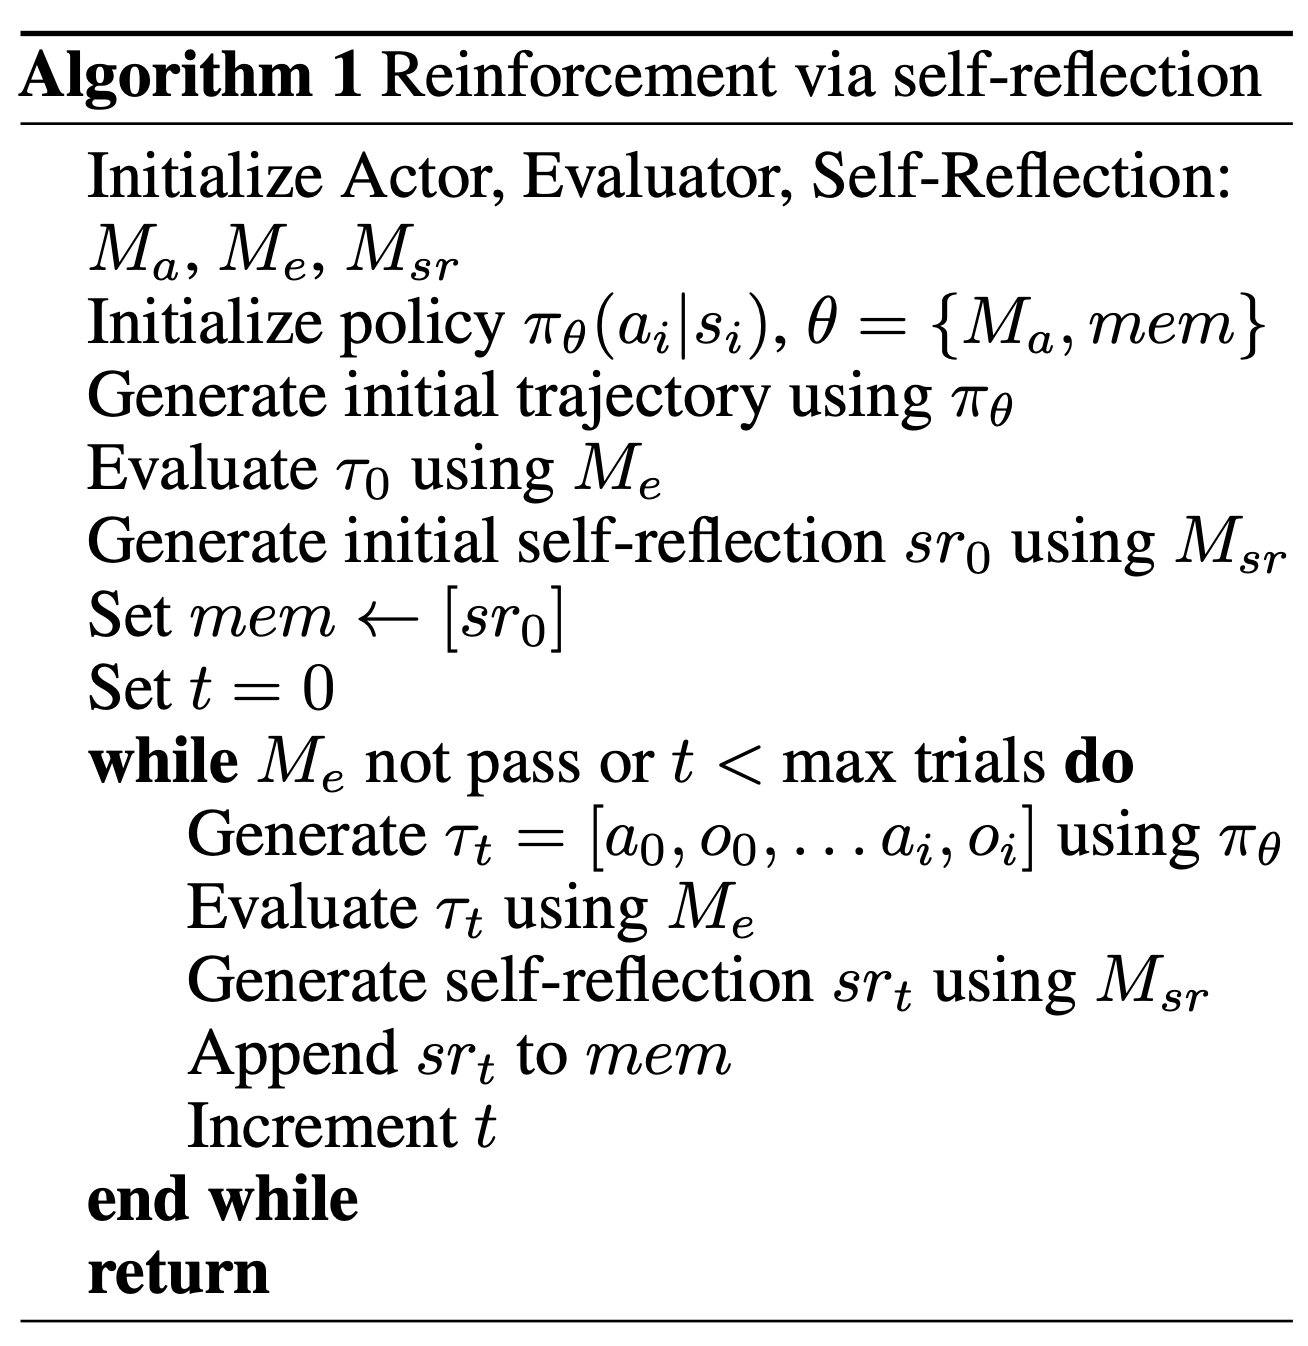
\includegraphics[width=0.5\linewidth]{figures/reflexion-code.png}
    \caption{Reflexion Algorithm \citep{shinn2024reflexion}}
    \label{fig:reflexion-code}
\end{figure}

Figure~\ref{fig:reflexion-alg} shows the general concept of reflexion, the different prompts, and the different types of memory. Figure~\ref{fig:reflexion-code} shows the code of reflexion, with the different calls to the LLM in line 3, 5, and 6 ($M_a$, $M_e$, and $M_{sr}$) and line 9, 11, 12. Note that the code is pseudo code, with important details about memory management, prompt management, and convergence criterium left open. 
Have a look at the repository in Github for details. 

Reflexion uses the same LLM with different prompts, which may lead to learning instability, and loops. Furthermore, memory management is relatively simple, with the potential of context overruns. An idea is to implement chunking or other memory compression methods, by hand in Python, or using an LLM.

First play with the reflexion repository, try to get it to work on the reflexion application, such as AlfWorld and HotpotQA. 

\paragraph{Extensions}
Now, try to implement a reflexion agent in BALROG, to run on the BALROG benchmarks.
What problem do you encounter? Does reflexion improve performance over the standard BALROG agents? 

Next,   extend the problem further. You can  try to find other reflection methods in the literature, or try to create new reflection methods from your own. You can try different   application types, and you can try to see how your approaches perform. And you can of course try  other LLMs.

\section{Concluding Remarks}
In this chapter we have discussed a practical case study, to see how an LLM can performs self-reflection. We used BALROG, a popular benchmark suite for reasoning tasks. BALROG consists of a mix from easy to hard games, some of which are difficult for LLMs to play well.
The BALROG suite is designed in an open style. We can write our own agent code that can then be run on the BALROG games. 

This has been an important practical case study. 
You have explored writing our own agent code for in-context reasoning. You have also gone beyond base-learning, by implementing self-reflection. You have explored the stability of self-reflection, on different LLMs and with highly challenging benchmarks.

%In this chapter, you have gained experience with state of the art problems in the field.
%
%The field is young, and not all problems have been resolved. LLMs are powerful, but there are certainly problems that they cannot solve. Some of these problems are planning related, such as the problems in the BALROG suite. This is an active area of research, and new methods will be invented that will perform better on planning problems. Another challenging problem is the knowing-doing gap. This is also an active area of research.





\begin{comment}
    
Set API-key

Choose configuration parameter.

go to naive agent

\begin{enumerate}
    \item Read the BALROG paper to understand the point of the benchmark
\item First decide on running locally and setting up your infrastructure.
\item Second install BALROG.
\item Third try to run the example code, generate graphs, check them with the paper.
Run it for the simple benchmark, and for the harder ones, to get a feeling for the problem that BALROG agents are meant to address.
\item Write a simple custom agent. Perform experiments. Does it solve simple benchmarks? Harder ones?
\item Write a more elaborate agent, for example based in Tree of Throughts, or ReAct. See how it performs on easy and on hard benchmarks. Does it do self-reflection?
\item Write a metalearning approach. What does it mean to do metalearning in a gaming environment? What is the inner loop, what is the outer loop?
\item Can you think of even more elaborate self reflection approaches?
\end{enumerate}


\subsection{Agent Development}

Run the planning agent.

implement prompt improver.

Look at tutorial

Implement ReAct

\end{comment}


\bibliographystyle{plainnat}
\bibliography{agenticbook,refs,case,synthetic}
